\section{\gls{ims} dataset No.3 - Bearing 3 sensor}
\label{sec:IMS_n3_3x}

\subsection{\gls{nd} instance}

In the previous section about the \gls{ims} dataset No.2, the framework capability for detecting novelties and known faults has been tested. The third dataset exploits the same fault as the second dataset. This enables testing the framework capability on detecting novelties and known faults on a new bearing, without retraining the model from scratch. In this case, the outer race failure is experienced by Bearing 3, so the sensor declared in the configuration file is the one for this bearing.

Running the \gls{mla} in evaluation mode, the novelty metric computed for the first 300 \gls{glo:snap}s of the dataset, is shown in \autoref{fig:IMS_n3_3x_nd}. All the \gls{glo:snap}s are considered novelties. This means that the new bearing behaves differently from the previous ones. 

\begin{figure}
    \centering
    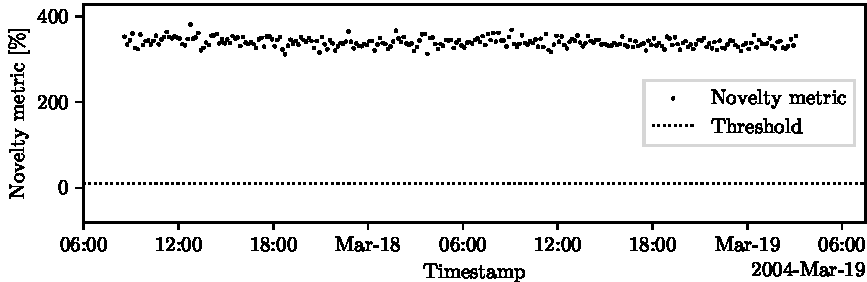
\includegraphics{images/IMS/Test03/retrain.pdf}
    \caption{Novelty detection on the \gls{ims} dataset No.3 using the sensor of Bearing 3, and the previous model trained on the dataset No.2}
    \label{fig:IMS_n3_3x_nd}
\end{figure}

The \gls{mla} saved all these \gls{glo:snap}s in the \emph{quarantined} collection. At this point, the \gls{mla} is switched to re-training mode, and the \emph{quarantined} collection is used to update the model. The silhouette criterion suggested using 2 \gls{glo:clust}s. Since the previous model was already trained with two \gls{glo:clust}s, this means that the new training data are assigned to existing \gls{glo:clust}s, enlarging them, instead of generating a new \gls{glo:clust}. 

The updated model is then switched to evaluation mode. The novelty metric computed for the rest of the dataset is shown in \autoref{fig:IMS_n3_3x_nd_updated}. The \gls{nd} event is triggered at 2004-04-12 19:21, $\approx$ 5~days before the end of the data acquisition. After the event, the novelty metric returns to the same level as before the event for two more days, before increasing again over the threshold and remaining consistently over the threshold.

\begin{figure}
    \centering
    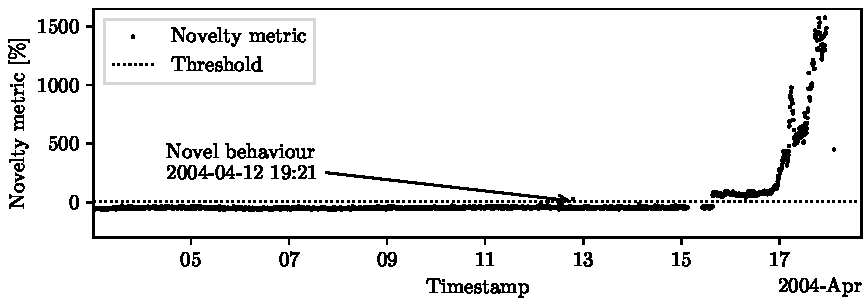
\includegraphics[width=\textwidth]{images/IMS/Test03/ND.pdf}
    \caption{Novelty detection on the \gls{ims} dataset No.3 using the sensor of Bearing 3, and the previous model updated}
    \label{fig:IMS_n3_3x_nd_updated}
\end{figure}

At this point, the \gls{rul} can be predicted. The predictions made considering the last 250~\gls{glo:snap}s of the dataset are shown in \autoref{fig:IMS_n3_3x_prediction}. The first prediction shown is made at the same time as the \gls{nd} event. Even with only two \gls{glo:snap}s exceeding the threshold, the fitted curve is correctly diverging. This first \gls{rul} prediction is quite accurate. The second fit in the figure is made when the novelty metric started to increase abruptly, so it results in a very short \gls{rul} prediction, shorter than the actual remaining time of the dataset.

\begin{figure}
    \centering
    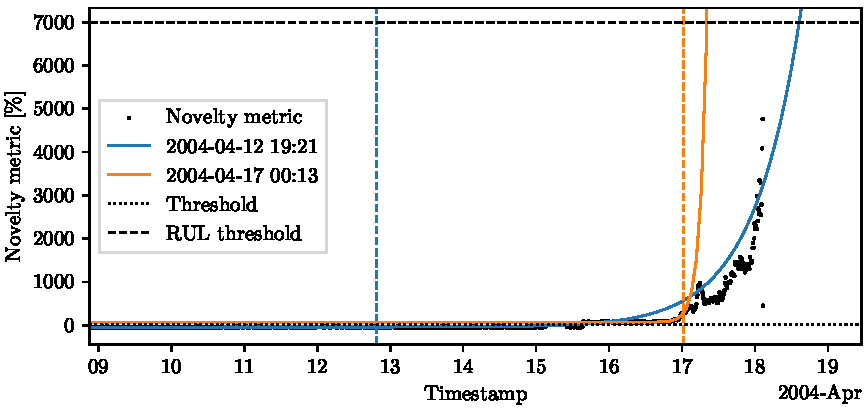
\includegraphics[width=\textwidth]{images/IMS/Test03/RUL.pdf}
    \caption{\gls{rul} prediction at different instants after the \gls{nd} event (dashed lines are the instants of the predictions corresponding to the same-colour solid line prediction)}
    \label{fig:IMS_n3_3x_prediction}
\end{figure}

\subsection{\gls{fd} instance}

The same test done for the \gls{nd} instance, can be repeated for the \gls{fd} instance of the \gls{mla}. The threshold is the same as for the previous test on dataset No. 2. The framework is set in fault evaluation mode, and all the dataset is analyzed. 

The fault score evolution over time is shown in \autoref{fig:IMS_n3_3x_fd}. 
The \gls{fd} event is triggered at 2004-04-17 17:33, hours before the fault.
An increasing pattern appears quite before the \gls{fd} event, and before that, the metric is very steady. This allows lowering the threshold to trigger the \gls{fd} event earlier.

Another observation about the fault metric is that, even at its maximum value, it remains still negative. This means that the pattern in the feature space becomes closer and closer to the fault \gls{glo:clust}, as time passes, without actually entering the \gls{glo:clust} boundaries.

\begin{figure}
    \centering
    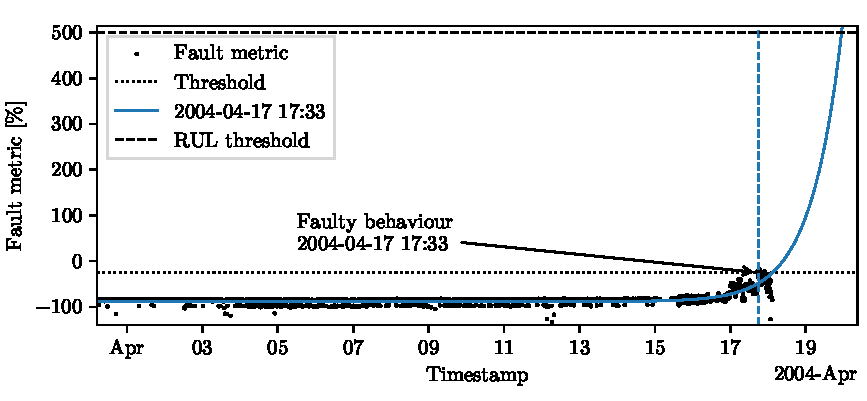
\includegraphics{images/IMS/Test03/FD.pdf}
    \caption{Fault detection on the \gls{ims} dataset No.3 using the sensor of Bearing 3}
    \label{fig:IMS_n3_3x_fd}
\end{figure}